\chapter{Enabling Process-Level Migration in Open MPI}
\label{cap:design}

The software implementation proposed in this thesis can be split in two parts.
The first one - subject of this chapter - is the implementation of the
\texttt{mig} framework and the related changes in Open MPI. The second one -
presented in Chapter \ref{cap:integration} - is the
integration of Open MPI with Barbeque Run-Time Resource Manager, including a
resource management policy that exploits the migration mechanism introduced.

\section{Process migration flow design}

The migration mechanism proposed is integrated in the Open MPI as a novel
framework, leaving to the
resource manager the implementation of the logic according to which is it
worth to require a migration to Open MPI. The idea is
to relieve the MPI framework all the aspect of resource management, fault
tolerance and other tasks that would be better performed by an external
manager. The resource manager may have a wider visibility on the
overall distributed system (or cluster) and may consider also non-MPI
application in the resource accounting.

The core idea of the proposed migration technique is to be as much as
possible transparent not only with respect to the applications, but also to
other Open MPI frameworks, consequently proposing a system-level and
process-level migration. At the time of writing the number of frameworks is
over 50, each of them having between 1 to 10 components. The last consideration
is the main reason to guarantee the maximum
transparency with respect to other frameworks and it is one of the key
differences
with previous system-level approaches in C/R and migration in Open MPI and it
ensures simplicity and maintainability of the proposed solution.

Our migration mechanism consists of migrating not the single MPI process, but the
overall \emph{ORTE daemon}. This means that the migration involves batch of Open MPI
processes, in first approximation all processes in each node. Subsection 
\ref{subsec:multipleorted} contains further discussions about the migration
granularity. 

\begin{figure}[t!]
		\centerline 
{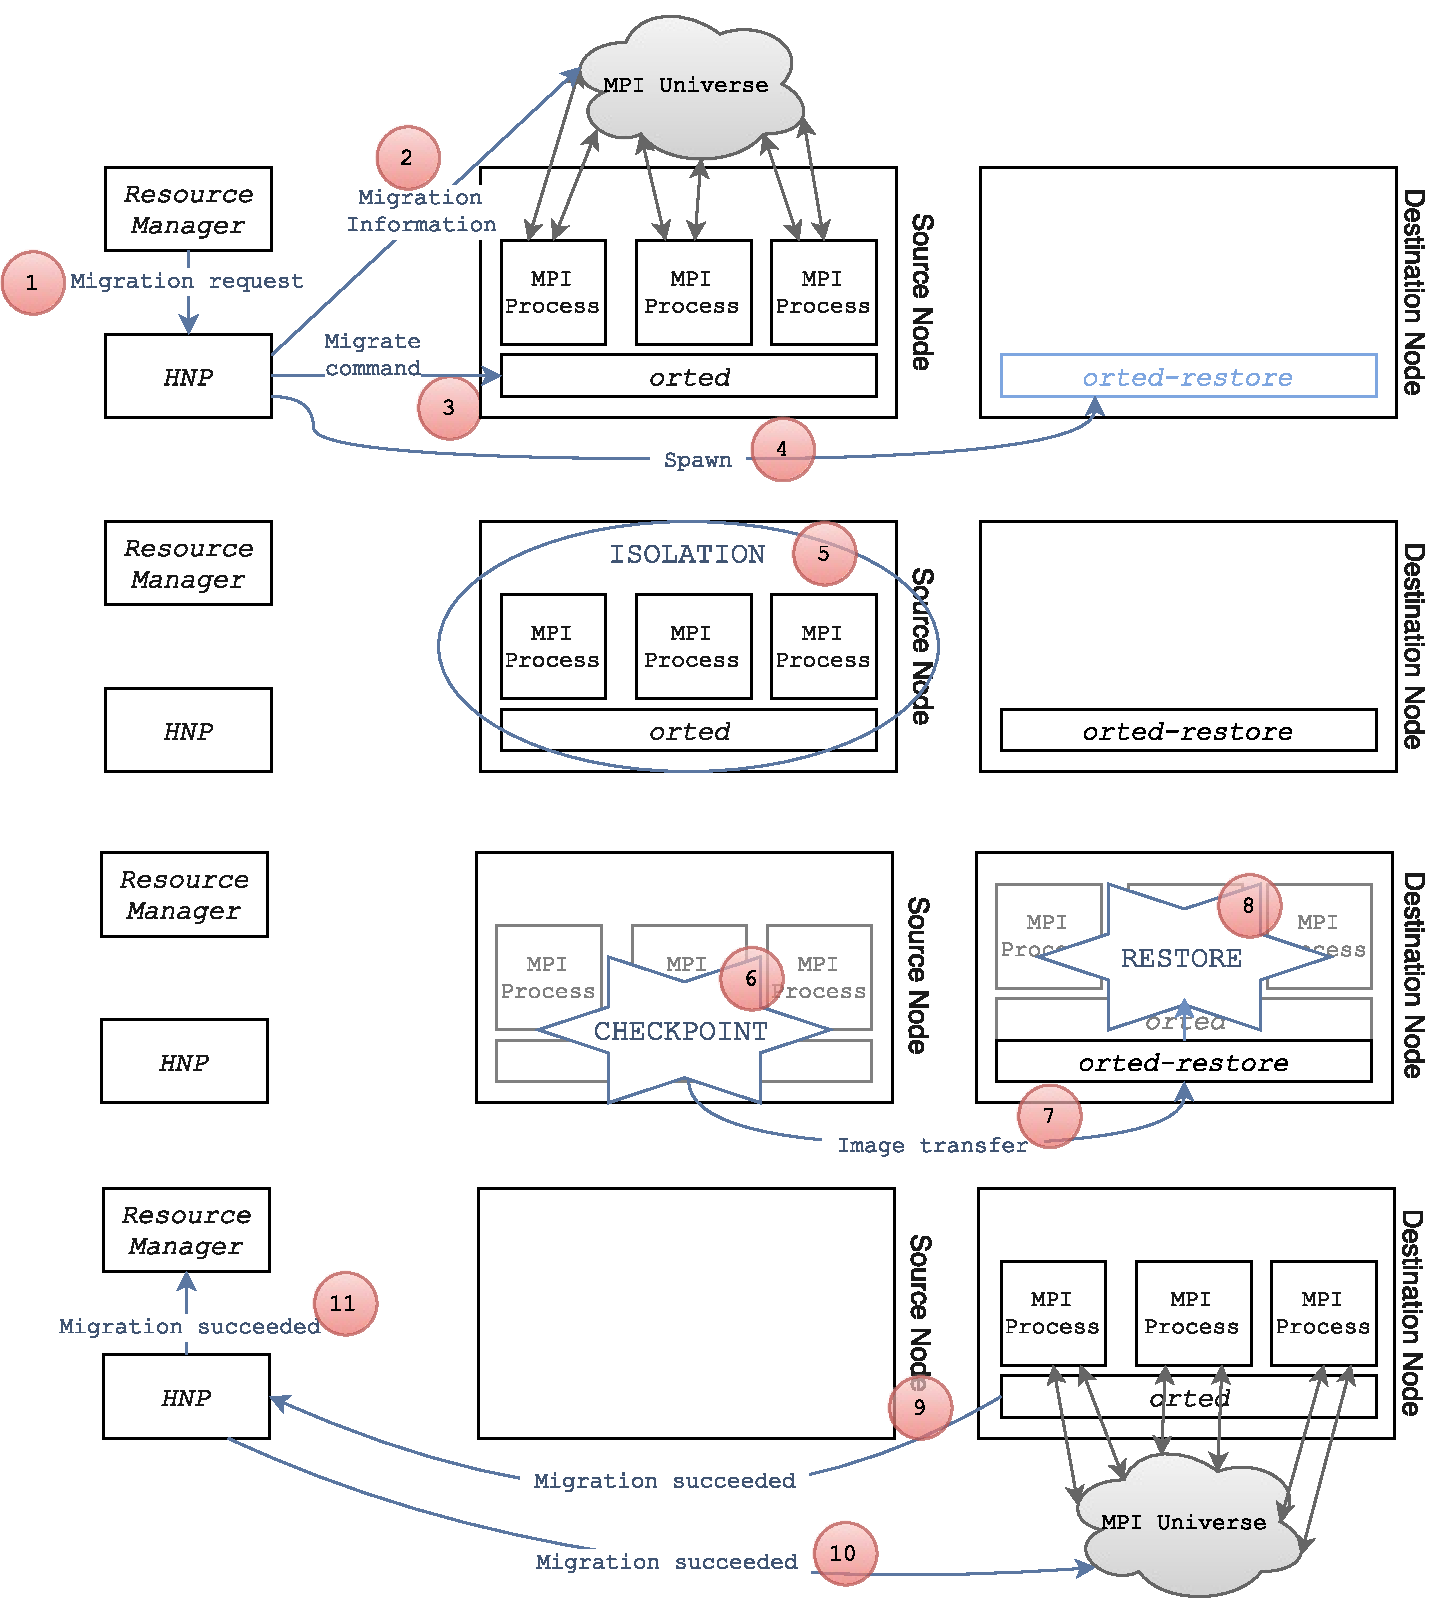
\includegraphics[scale=0.55]{img/cap4-migdescription.pdf}}
		\caption[The \texttt{mig} mechanism]{Description of migration mechanism implemented through the \texttt{mig} framework.}
		\label{fig:cap4-mighighlevel}
\end{figure}
%\clearpage

Following the flow depicted in Figure \ref{fig:cap4-mighighlevel}, the designed
sequence of migration is:
\begin{enumerate}
\item The resource manager asks a migration to the HNP;
\item The HNP informs all \emph{ORTE daemons} and for extension all MPI processes;
\item The HNP issues the migration command to the \emph{ORTE daemon} on node
      requested to be migrated;
\item Simultaneously with the previous command, \texttt{orted-restore} is spawned in
      the destination node (see Subsection \ref{sub:orted-restore} for details);
\item The migrating \emph{ORTE daemon} issues the command to own processes to
      isolate themselves with respect to remote MPI processes;
\item The checkpoint is performed;
\item The resulting image state is transfered to the destination node;
\item The \texttt{orted-restore} performs the restart;
\item The restarted \texttt{orted} informs the HNP of the successful migration;
\item The HNP notifies all other processes about successful migration. They
      starts the restoring of the connections;
\item The HNP notifies the resource manager about successful migration.
\end{enumerate}

To actually execute the steps 6 and 8 the Checkpoint/Restore In Userspace
(CRIU) tool is used, as described in next Subsections. The most
important overhead is the step 7, as subsequently confirmed by the benchmark
presented in Chapter \ref{cap:evaluation}.

\subsection{Multiple ORTE daemons on the same node}
\label{subsec:multipleorted}
The migration mechanism works at \texttt{orted}-level and this entails the
limitation of moving only the entire set of processes assigned to a node.
Therefore, it is not possible to move a single process.

In order to mitigate the previous limitation, we added to Open MPI the
capability
to spawn multiple \emph{ORTE daemons} on the same node. This is not usually
desired since two processes in the different \emph{ORTE daemons} cannot
communicate via shared memory, but they need to use \emph{TCP} or other network
protocol. However, network protocols routed in local does not impact
significantly. The overhead introduces will be analyzed in Section
\ref{cap:evaluation}.

In HPC oriented systems, even a small local overhead may have a not negligible
impact
on the execution of parallel applications on multiple nodes.
 However, migrating with the granularity of \emph{ORTE daemon} presents
several advantages for process migration:
\begin{itemize}
\item The MPI processes does not need to change the active component used in 
      communication. If two processes are spawned by the same \emph{ORTE daemon}
      they communicate via shared memory and after migration they are still able
      to communicate via shared memory. Vice versa, if two processes are in
      different \emph{ORTE daemon} groups, they communicate via network (e.g. 
      TCP) and they still use that network (e.g. TCP) after the migration of one
      of \emph{ORTE daemon};
\item It is not necessary to close and reopen the communication channels between
      \emph{ORTE daemon} and its MPI processes, i.e. the POSIX pipes. The CRIU
      framework guarantees that they will properly work also after the restore;
\item The Open MPI internal states have to be changed in a minimal part.
      Assuming all nodes homogeneous, the most important parameter that will
      change after migration is the IP address of that daemon and processes.
      Other information that will change are the hostname, the domain name, etc;
\item Most of the Open MPI frameworks, as well as the applications, are
completely
      un-aware of the migration. They notice only a long delay in the
      communication network from and towards the migrating processes.
\end{itemize}

\subsection{The \texttt{orted-restore} helper program}
\label{sub:orted-restore}
After the checkpoint of the source \emph{ORTE daemon} the image has to be
transfered on the destination node. Subsequently, the \texttt{orted} has to be
restarted via the appropriate CRIU API calls. 

Initially, we thought about using \texttt{ssh}: a connection from the source node to
the destination node is used to copy the image in the new node and another
connection from \emph{HNP} to destination node would issue the command necessary
to the restart. However, this idea was put aside due to the large overhead of
\texttt{ssh} connection, both for the connection latency and for data encryption
overhead. A standard AES256-CTR chiper may easily halve the throughput
\cite{rapier2008high}.

Currently, the image transfer is performed in plain-text via TCP socket between the
\emph{ORTE daemon} and the program \texttt{orted-restore} spawned on the
destination node for this purpose. The \texttt{orted-restore}
has also the task of invoking the restart function of CRIU. Once the 
migrating \texttt{orted} and its processes are successfully restarted, the
\texttt{orted-restore} waits for their termination before exiting.

In order to spawn the \texttt{orted-restore} on the remote machine, the
\texttt{mig} framework relies on the \texttt{plm} framework functions. The
\texttt{plm} spawns the \linebreak \texttt{orted-restore} using the same method used
to spawn the \emph{ORTE daemons}. Currently, we implemented the functionality
only for \texttt{ssh} component of \texttt{plm} - the most used one -, anyway
it's easy to extend other components to support this feature.

We decided to implement also the possibility of compressing the image before the
transfer. The performance measures presented in the Chapter
\ref{cap:evaluation} reveal that for the most HPC applications, compress the
image does not give any advantage. The resource manager is in charge of
choosing between compressing or not the image. 

\subsection{The global consistent state}
As previously discussed in Section \ref{sec:CRApproach}, a \textbf{Global
Consistent State} is typically reached by the existing C/R tools before
performing the Checkpoint of the application.

In our implementation a \emph{Global Consistent State} is simply never reached.
Since we are interested in achieving the maximum transparency with respect to the
application with the minimum migration overhead, reaching a safe-point by all
MPI processes is an avoidable feature. Furthermore, processes not involved in
migration are able to continue execution if they do not require to communicate
with migrating processes.

Even if a \emph{Global Consistent State} is not reached, the correctness of the
application is guaranteed by the fact that no messages
are lost during the migration. This is enforced thanks to a careful
coordination of the migration and the modifications applied to \texttt{btl}
described in next sections.

\section{Open MPI modifications}
\subsection{The \texttt{mig} framework}
The \texttt{mig} framework, shorten for \emph{migration}, is the new framework
added by this work. It is the core of migration mechanism both in HNP and in
processes. Part of the framework is executed only in HNP and it has the role of
coordinating all the migration phases. Other functions are executed only in
the \emph{ORTE daemon} (e.g. the CRIU calls) and others only in the MPI
processes (e.g. to perform the IP address changes).

\subsubsection{Components}
The framework has several common functions in the \texttt{base} component while
other components provide the Checkpoint/Restore functionalities. Currently only
the \texttt{criu} component is present, since we selected CRIU to perform the
C/R of processes.

The functionalities provided by the base component may be overwritten by the
active component. At present, the functionalities of \texttt{criu} component are
complementary to the \texttt{base}, thus no overwrite is necessary. The
\texttt{base} components provides:
\begin{itemize}
\item The entry point function called by \texttt{ras} to start the migration
      procedure;
\item The exported callback function that \texttt{plm} will use when a migration
      message is incoming;  
\item A function called by the HNP, in
      order to refresh the data changed after migration, e.g. the hostname of
      migrated \emph{ORTE daemon};
\item The image transfer functions between the migrating \texttt{orted} and the
      \linebreak
      \texttt{orted-restore} on the destination node; 
\item The timing to perform benchmarks on the migration mechanism.
\end{itemize}

Instead, the \texttt{criu} component implements the API calls to CRIU, 
in order to actually perform the Checkpoint and the Restore of MPI
processes.
These functions are never executed in the MPI processes, but only in the
migrating \texttt{orted} and in the \texttt{orted-restore} executable.

\subsection{Other frameworks}
Besides the newly introduced \texttt{mig} framework, the migration mechanism
required the modification of other already existing frameworks.
These changes are not very
intrusive and usually they have been added in separated source files, with the exception of the
\texttt{btl} framework, that required several injected lines of code.
This separation guarantees a good level of maintainability.

Changes required for enabling the migration mechanism have been introduced in:
\begin{itemize}
\item \texttt{ras} (part of ORTE): currently, Open MPI uses
this framework only in the application initialization, to get the full list
of available nodes.
We extended the \texttt{ras} API to allow the resource manager to send
migration requests during the applications execution and to be notified
about the status of the requests.

\item \texttt{oob} (part of ORTE): the ``out-of-band'' framework provides the
low-level API for the communication between HNP $\Leftrightarrow$
\texttt{orted}, and \texttt{orted} $\Leftrightarrow$ its child processes.
The current Open MPI implementation includes TCP as the only transport layer for
\emph{ORTE daemons} inter-communication. This framework contributes to the
process migration by managing the opening and closure of the pending
TCP socket connections towards the migrating \emph{ORTE daemon} instance.

\item \texttt{plm} (part of ORTE): high-level HNP
$\Leftrightarrow$ \texttt{orted} communication framework. We implemented
the protocol necessary to coordinate the \emph{ORTE daemon} instances in the \emph{base}
component. We also added the \texttt{ssh} call that spawns the \texttt
{orted-restore} daemon on the destination node. This daemon is in charge of
resuming the processes execution once the checkpoint image transfer is
completed.

\item \texttt{btl} (part of OMPI): this is the application-level peer-to-peer
communication framework. In our work we modified the \emph{TCP} component to
manage the opening/closure of the TCP socket connections among migrating
application processes. See Section \ref{sec:btlcoord} for details.

\end{itemize}


\section{The migration phases}
\label{sec:cap4-migphases}
\begin{figure}[t]
		\centerline 
{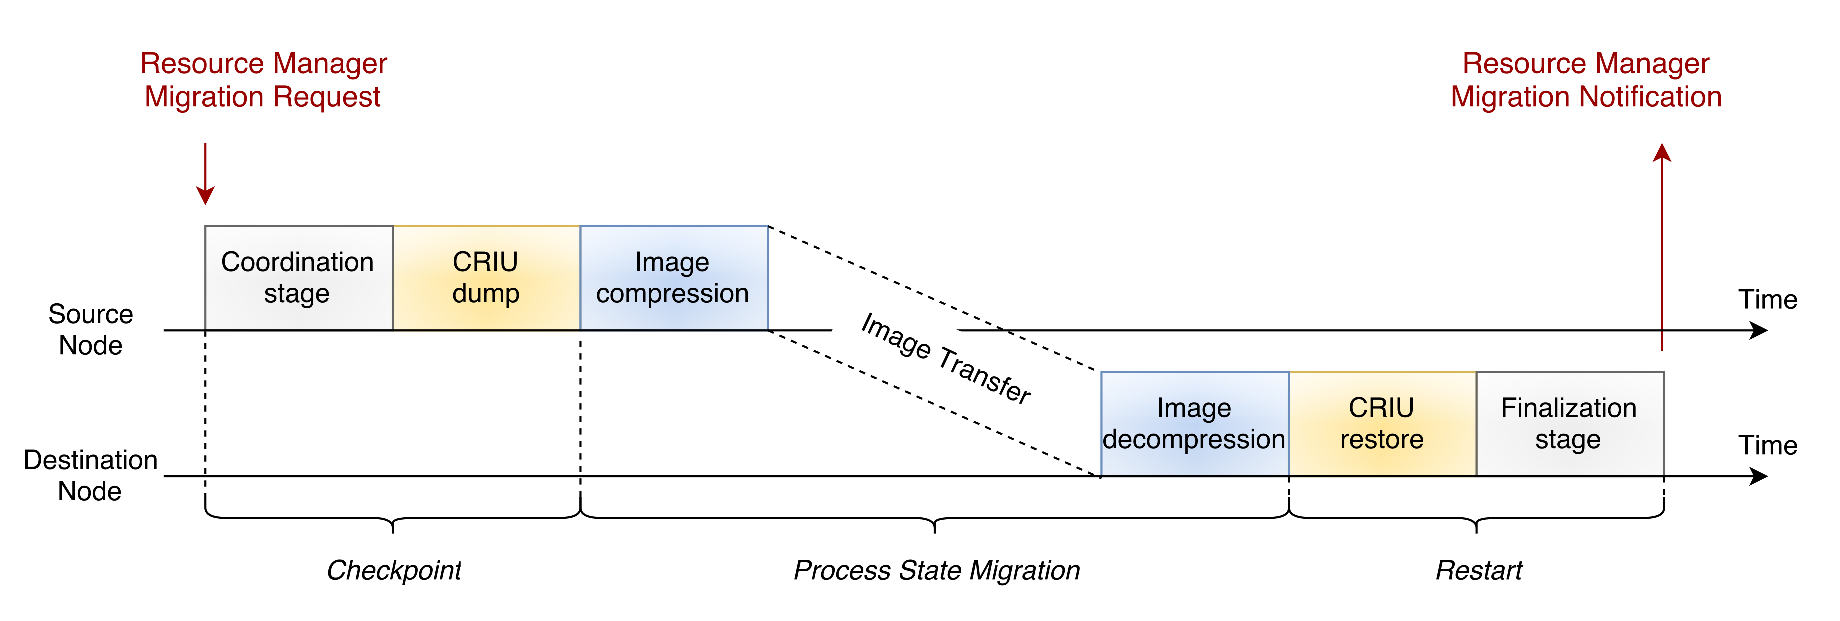
\includegraphics[scale=0.43]{img/cap4-phases.eps}}
		\caption[The migration phases]{The migration phases.}
		\label{fig:cap4-migphases}
\end{figure}

This section describes in detail how the proposed migration mechanism
is structured. We have divided the migration procedure in five phases:
\begin{itemize}
\item Coordination stage;
\item CRIU dump;
\item Process state migration;
\item CRIU restore; 
\item Finalization stage.
\end{itemize}
This schema is shown in Figure \ref{fig:cap4-migphases}.

\subsection{Coordination Stage}

The coordination stage starts when the \texttt{mig} framework on the Head Node Process
receives from \texttt{ras} a migration request specifying a source and a destination nodes.

The \texttt{mig} framework spawns an \texttt{orted-restore} daemon on the
destination node, which is therefore able to receive the migrating ORTE
daemon. Then, via \texttt{plm}, the framework issues a \texttt{MIGRATION\_PREPARE}
command to all the ORTE daemon instances running over the system, broadcasting
the information related to the migration request.
When the ORTE daemon instances receive the command, they notify the request to
their children (the application processes) using the signals provided by
Linux-OS\footnote{Open MPI developers have planned to release the
\texttt{pmix} framework, which allows the ORTE daemon to communicate via Unix
sockets to its children. Our approach will be changed accordingly}.

The signal handler, implemented in the OMPI library, intercepts the\\\texttt
{MIGRATION\_PREPARE} signal/command. The \texttt{btl} TCP component of the
processes that are not migrating performs the
following actions: 
\begin{enumerate}
\item Caching of any future send request towards the
      migrating processes;
\item Terminating any ongoing data transmission (\texttt{send()} system calls)
      towards the migrating processes;
\item Flushing the transmission buffer;
\item Performing a \texttt{shutdown}
      system call on the transmission-side of the TCP socket.
\end{enumerate}

After that, the processes send back an acknowledgement to their own ORTE daemon
instances, ensuring that no further transmissions will be performed towards the
frozen processes. In turn, the ORTE daemons forward the acknowledgement to the
Head Node Process. This synchronization protocol, which is depicted in Figure
\ref{fig:cap4-cmdsequence}, is involved in all the subsequent phases.

\begin{figure}[t]
		\centerline 
{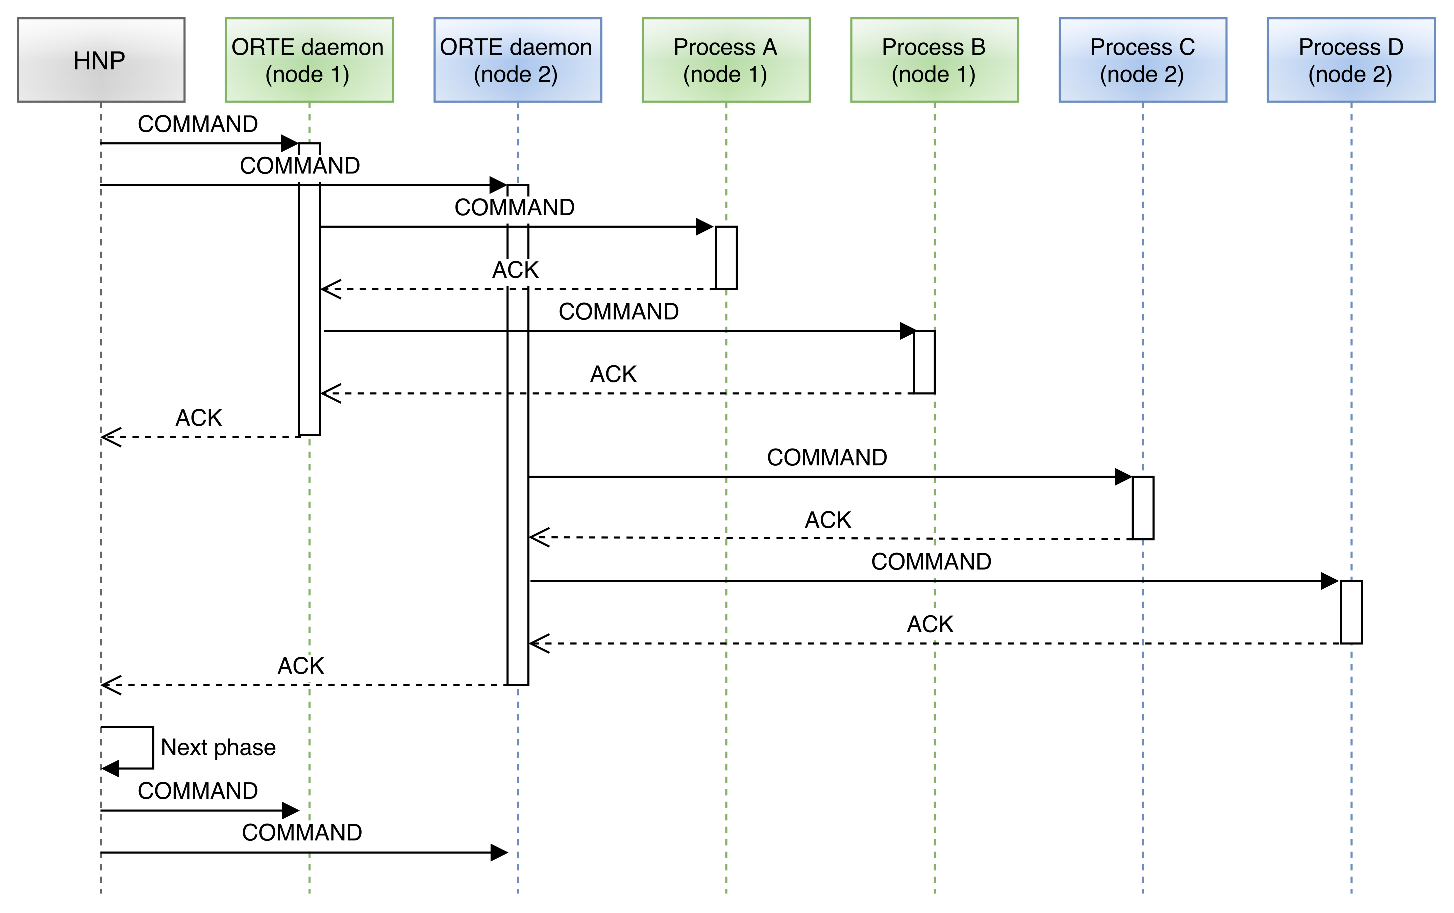
\includegraphics[scale=0.5]{img/cap4-cmdsequence.eps}}
		\caption[Migration messages exchange]{Sequence diagram migration messages exchange.}
		\label{fig:cap4-cmdsequence}
\end{figure}

\subsection{CRIU Dump (Checkpoint)}

Once all the ORTE daemon instances are aware of the migration request, the
Head Node Process
can issue the \linebreak \texttt{MIGRATION\_EXEC} command and effectively start the
migration procedure. When an application process receives the \texttt
{MIGRATION\_EXEC} command, it waits until all the in-flight packets have been
received by the destination side. At this point, all the TCP connections towards
processes involved in the migration can be safely closed, and an acknowledgment
can be sent back to the ORTE daemon.

When the migrating ORTE daemon receives the acknowledgment, it uses the API
provided by the CRIU library to perform the checkpoint of its execution status.
The checkpoint outcome, i.e. the generated process dump, is stored
in a temporary directory. Following the Open MPI common practice, the temporary
directory is set to \texttt{/tmp}. However, a problem may arise if \texttt{/tmp}
is mounted in the main memory (most common case) and the amount of memory
available is not enough to store the dump. To address this issue, the user or
the resource manager can specify a different directory.


\subsection{Process State Migration}

As previously described, the outcome of the CRIU checkpoint (or dump), i.e. the
process dump, is a collection of files. To simplify the transfer of such files
over the network, the next step is to create an archive containing such files
and optionally compress them. For brevity we are going to call the checkpoint
archive `'image''.

Generally, the decision of compressing or not the archive requires the
evaluation of the trade-off between compression time and transfer time savings
due to compression. This task can be in charge of the resource manager, which
should consider several factors, e.g. network bandwidth, network traffic, image
size, shared memory occupation and disk
performance.

The image is now ready to be moved to the destination node.
CRIU has a server functionality that allows the \emph{disk-less} transfer
the image.
However, at time of development this feature was not very mature and the C API
relative to the server is not complete. Therefore, we decided to do not use
the integrated CRIU server.

The transfer can be achieved according to two strategies: 
\begin{enumerate}
\item using a TCP connection between source and destination nodes;
\item using a Network File System (NFS).
\end{enumerate}
At the time of writing, we do not have a storage unit with NFS available for
testing, therefore we selected the TCP based option to transfer the image
between nodes.


\subsection{CRIU Restore (Restart)}

When the \texttt{orted-restore} daemon running on the destination node receives
-- and possibly decompresses -- the image coming from the source node, it
restarts the ORTE daemon and its children processes using the CRIU API.
Since the C/R approach of CRIU is totally transparent to the (frozen) processes,
after the restart we need to send a signal to the restored ORTE daemon
to advise it that a node migration has occurred. Accordingly, the ORTE daemon
reopens the connection to the Head Node Process and sends the \texttt{MIGRATION\_DONE}
message.

Finally, the Head Node Process broadcasts the \texttt{MIGRATION\_DONE} message to all
the other ORTE daemons and processes using the same synchronization protocol
previously described.


\subsection{Finalization Stage}

When all the processes have received the \texttt{MIGRATION\_DONE} message, the
migration procedure enters the \emph{Finalization stage}. In this phase, to
minimize the overhead, the migrated processes reopen the connections towards
other processes only if needed. This happens if there are packets waiting in the
buffer or if the application has new data to transmit.

Once again, it is worth underlying that the entire migration procedure is
performed without the awareness of the application, which only experiences
a network delay in the communication towards migrating processes.

Moreover, the performance degradation is additionally mitigated by having all
the nodes not involved in the migration still communicating between each
other. In such a way, we avoid using complex algorithms to reach a global
consistent state. This is
another key advantage of our solution, since in application-level C/R schemes
the coordination phase presents several problems on both user and framework
sides \cite{schulz2004implementation}.

\section{The \texttt{btl} TCP component}
\label{sec:btlcoord}
This section shows the details on how the coordination between MPI processes
is performed, when they are using the \texttt{tcp} component of \texttt{btl}
framework. The \texttt{btl} framework is used exclusively by the MPI processes
to communicate with other processes in the application universe.

The \texttt{tcp} component exposes several functions used by other Open MPI
frameworks to send/receive messages and to open/close the communication towards
processes. The functions are always non-blocking: a callback function is
provided by the caller and it is called when the requested operation terminates
successful.

\subsection{The TCP endpoints}
Each process is identified by one \textbf{endpoint}, i.e. a data structure
containing several information, like the socket file descriptor, the high-level
reference of the process, the connection status, etc. The \emph{endpoint}
contains also the data fragments waiting to be processed in both directions.
A process has only one valid endpoint towards the same process.
The \emph{endpoint} may be in these status:
\begin{itemize}
\item \textbf{Closed}: the endpoint is closed and there is no active attempt to
                       connect to the process. Typically this is the case when
                       no messages are sent towards that process yet.
\item \textbf{Connecting}: the \texttt{connect} system call is trying to contact
                           the receiver.
\item \textbf{Connect Ack}: the \texttt{connect} system call has successful
                            established the connection towards the process,
                            however it's waiting the confirmation \emph{ack}
                            message. Open MPI implements a three-way
                            handshake-like protocol.
\item \textbf{Connected}: the node is connected and ready to send/receive
                          messages.
\item \textbf{Failed}: an error has occurred and the socket is no more
                       available. Usually this condition leads to an unstable
                       condition that in turn leads to the application crash.
\end{itemize}

In order to perform the migration, we add the \textbf{Frozen} to the
possible endpoint statuses. This status is used to identify the \emph{endpoint}
condition towards the migrating processes or, if it is the migrating process
itself, the conditions of all others \emph{endpoint} not in the local
\emph{ORTE Daemon}.

The \emph{Frozen} status is used to provide a sort of ``lock`` on the endpoint.
Next calls to send, receive and similar functions stacks the outcoming messages
to a queue of fragments to be sent. This queue will be flushed only when the
migration has occurred and the processes resumed. The send caller does not
notice any difference with respect to a normal send, but only a long delay on
the execution of the callback function.

\subsection{Freezing the connections before migration}
The \texttt{base} component of \texttt{btl} framework provides the interface
with the \emph{ORTE Daemon}. At present, it uses a sequence of signals to
coordinate with the daemon. Then, it calls the \texttt{mig\_event} functions
exposed by the active \texttt{btl} components, in our case the \texttt{tcp}
component.

The \texttt{tcp} component will perform the freeze of all involved endpoints
(endpoints of migrating processes if it is a non-migrating process, all
endpoints of non-migrating processes if it a migrating processes). Then it will 
send
back to the \texttt{base} component the confirmation, which will be forwarded
to the \emph{ORTE Daemon}.

Freezing the \emph{endpoints} entails also ensuring that no in-flight messages
are present. In order to ensure this, each process initially closes
only the trasmission-side of the socket. Subsequently, it waits that the other
side closes its trasmission-side, in this way the \texttt{recv} system call will
fail. Then the \texttt{recv} system call fails, the socket can be safely closed
and the migration ack can be sent back to the \texttt{base} component.

\subsection{Restoring the connections after migration}
When the migration ends, the \texttt{base} component calls again the
\texttt{mig\_event} functions. The statuses of frozen \emph{endpoints} are
changed to \emph{Closed} and the connections are restarted only if there are
fragments waiting in the queue. If the queue associated to the \emph{endpoint} is empty, the
connection is not restored immediately, in order to limit the congestion due
to the reconnection of other processes. The connection will be re-established
only when the first message arrives via the \texttt{send} call.

It may happen that two processes try to re-establish the connection
simultaneously. In this case, the \texttt{tcp} component will recognize this
scenario and close one of the two connections, actually using only one
connection in a full-duplex mode.


\section{Solving system resource conflicts on restart}
The restart stage is not straightforward if it occurs on a node different from
where the Checkpoint has been performed. Program executable, libraries and
data files must be in fact present and identical in the destination node.
Moreover, remote file-systems must be mounted and the process identification
numbers (PIDs) must be available because the processes cannot change their
PIDs after the restore. Given that, there is no guarantee about the fact that
the PIDs of the migrating processes have not been already assigned on the
destination node.

CRIU does not allow to migrate processes having opened device files,
established network sockets with different machine, \texttt{O\_DIRECT} pipes,
etc. (the full list can be found in the CRIU documentation). 

In order to solve all the above mentioned issues the \texttt{orted-restore}
performs specific system calls in order to isolate the processes in different
\emph{Linux Namespaces}. The \textbf{Linux Namespaces} allow an application to fork children in a detached environment. 

\subsection{Linux Namespaces}
\textbf{Linux Namespaces} is a Linux kernel feature that provides an 
abstraction of system resources, such that processes within a namespace run in
a isolated environment. The changes to the system resources inside a namespace
are visible
only to other processes members of that namespace.
They are described in the \emph{Overview, conventions, and miscellaneous}
(Section 7) of the Linux Programmer's Manual \cite{LinuxNamespaces}.
The available namespaces are:
\begin{itemize}
\item \textbf{CGroup} \cite{cgroupdoc}: isolation of Control Groups, providing
a different \linebreak \texttt{/proc/self/cgroup} file for each namespace;
\item \textbf{IPC}: POSIX message queues and other inter-process communication;
\item \textbf{Network}: network devices, TCP/UDP ports, etc.;
\item \textbf{Mount}: the mount points;
\item \textbf{PID}: isolation of process identifiers; 
\item \textbf{User}: user and group identifier;
\item \textbf{UTS}: UNIX Timesharing System, it isolates the hostname,
domain name, etc.
\end{itemize}

In this work both the PID and the Mount namespaces are used.

The PID namespace, as already discussed, is necessary in order to guarantee
that the Process Identifiers of checkpointed processes are available on the
destination node. Instead, the Mount namespace is needed for more than one
reason:
\begin{itemize}
\item Detaching the Mount namespace is a pre-condition for detaching the PID
      namespace, since the \texttt{/proc} directory has to be remounted;
\item Open MPI uses the Linux \texttt{tty}s present in
      \texttt{/dev/} directory.
      These special files are created mounting the \texttt{devpts}
      pseudo-filesystem. To avoid conflicts with \texttt{tty}s already
      present in the system, the \texttt{devpts} has to be remounted,
      not for the entire system, but only to migrated processes;
\item Any other mountpoint, e.g. \emph{network filesystems}, may require the remount
      for the specific application.
\end{itemize}

\subsection{Unsharing the context}
To exploit the Linux Namespaces, the \texttt{<sched.h>} header provides the
\texttt{unshare} system call, that allows a process to detach part of its
execution context, associating it to other namespaces.

In our implementation, the \texttt{orted-restore} executes the following C call:

\vspace*{2mm}

\texttt{unshare(CLONE\_NEWNS | CLONE\_NEWPID)}

\vspace*{2mm}
\noindent

where the \texttt{CLONE\_NEWNS} flag detaches the mount namespace and the \linebreak
\texttt{CLONE\_NEWPID} flag detaches the PID namespace; hence,
\texttt{orted-restore} and its children share the new private namespaces.

The \texttt{orted-restore} daemon becomes then the \texttt{init} process
(PID=1)
in the new empty PID namespace of the destination node and can restart the
application processes with the original PIDs from the source node. The isolated
mount namespace is necessary to remount the \texttt{/proc} directory in order
to match the new process identifier configuration. At this point, the
\emph{ORTE daemon} instance and its children can be safely restarted.

The full stack of system calls required to restart the checkpointed
\emph{ORTE daemon} is described in Figure \ref{fig:cap4-unshare}.

\begin{figure}[t]
		\centerline 
{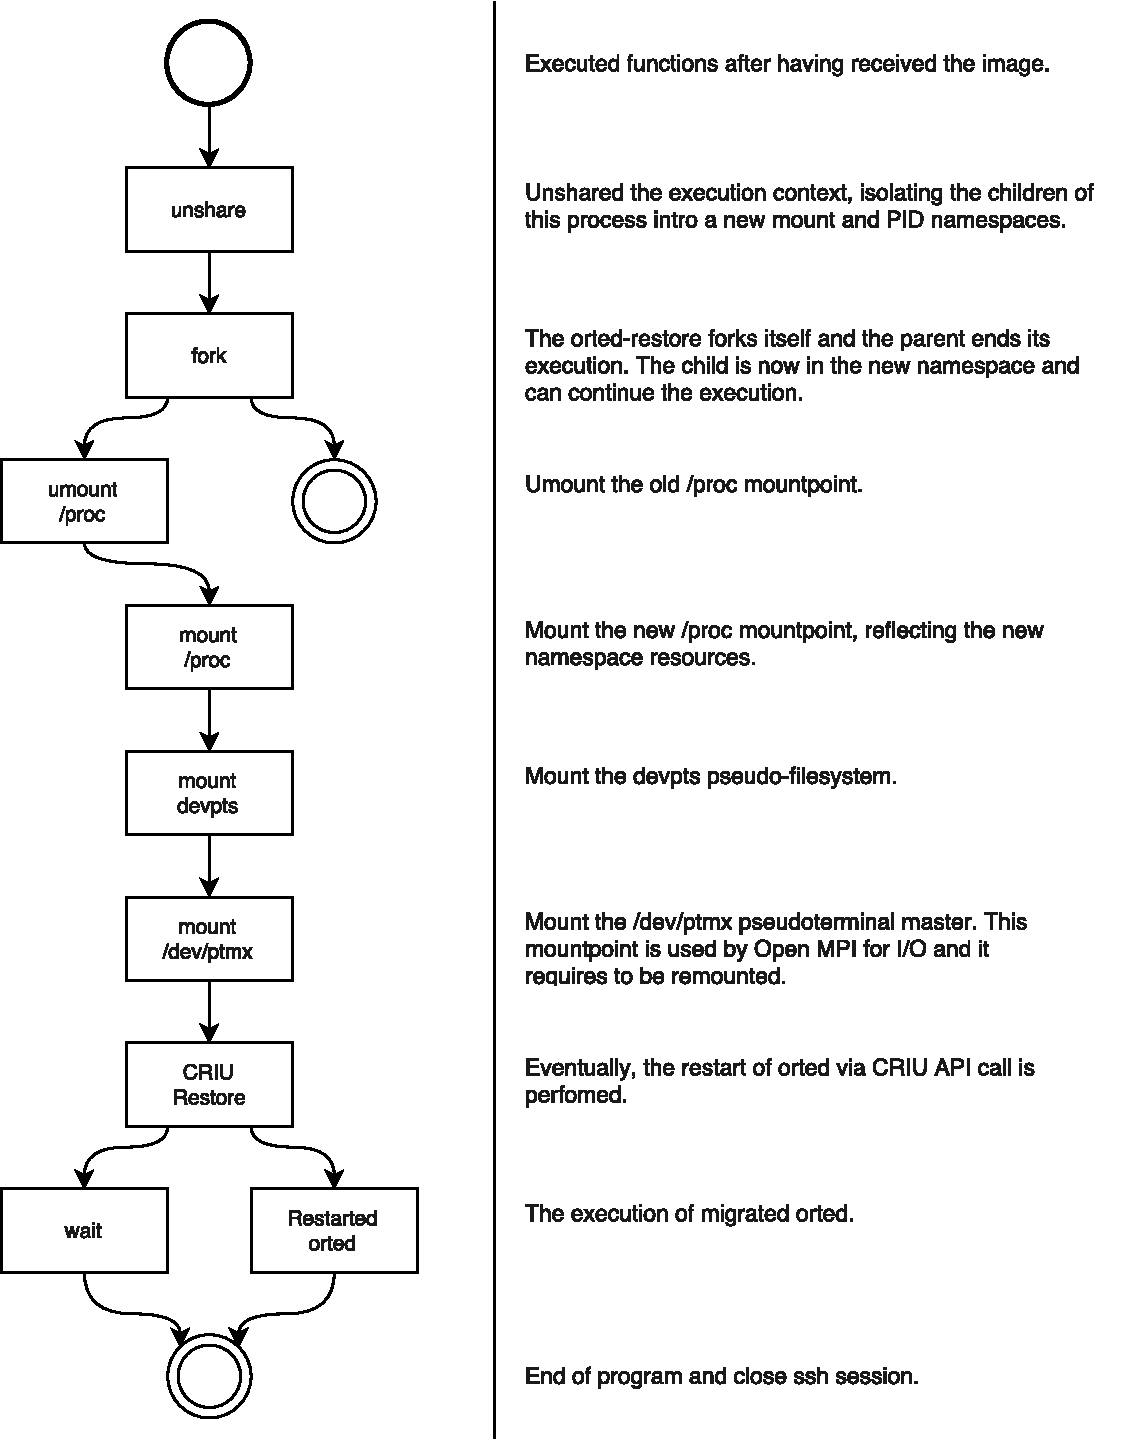
\includegraphics[scale=0.7]{img/cap4-unshare.pdf}}
		\caption[The \texttt{orted-restore} flow diagram]{Flow diagram of \texttt{orted-restore} execution.}
		\label{fig:cap4-unshare}
\end{figure}
